\chapter{实验数据采集方案与人口信息统计}
\section{引言}
数据是一切分析的前提与基础。由于目前暂无公开可用的PE生理信号数据库,数据来源问题是本研究亟需解决的基础性问题。鉴于此,本章首先阐述了临床研究方数据采集方案,对实验被试人员筛选标准、生理数据采集规范及数据导出流程等进行了介绍。
其次,本章也对第一章提及的多种孕妇PE风险因子以量表的形式进行了收集统计。最后,本章针对被试人员的除脉搏波外的数据进行了基本的相关性分析工作。
\section{数据来源}
\section{采集设备}
\section{采集流程}
\section{脉搏波数据导出}
\section{风险因子统计}
\begin{figure}[htbp]
    \centering
    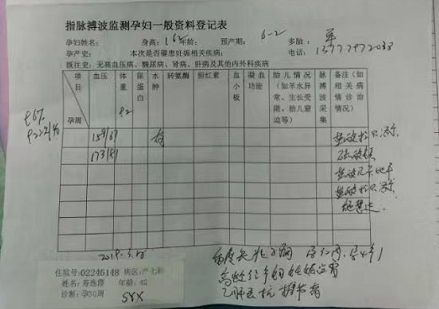
\includegraphics[width=.8\linewidth]{ch3/static}
    \caption{\label{fig:static}static}
\end{figure}


\begin{table}[htbp]
    \centering
    \caption{指端脉搏波监测孕妇一般资料登记表}
      \begin{tabular}{|r|r|r|r|r|r|r|r|r|r|r|r|r|}
      \multicolumn{1}{l}{孕妇姓名} & \multicolumn{2}{c}{} & \multicolumn{1}{l}{身高} & \multicolumn{2}{c}{} & \multicolumn{1}{l}{年龄} & \multicolumn{2}{c}{} & \multicolumn{1}{l}{孕产期} & \multicolumn{1}{r}{} & \multicolumn{1}{l}{多胎} & \multicolumn{1}{r}{} \\
      \multicolumn{1}{l}{孕产史} & \multicolumn{3}{c}{}  & \multicolumn{4}{c}{本次是否罹患妊娠相关疾病} & \multicolumn{2}{c}{} & \multicolumn{1}{l}{电话} & \multicolumn{2}{c}{} \\
      \multicolumn{7}{c}{既往史(有无高血压疾病、糖尿病、肾病、肝病及其他内外科疾病)}    & \multicolumn{6}{c}{} \\
      \midrule
      \multicolumn{1}{|p{4.19em}|}{孕周} & \multicolumn{1}{l|}{心率} & \multicolumn{1}{l|}{血压} & \multicolumn{1}{l|}{体重} & \multicolumn{1}{l|}{尿蛋白} & \multicolumn{1}{l|}{水肿} & \multicolumn{1}{l|}{转氨酶} & \multicolumn{1}{l|}{胆红素} & \multicolumn{1}{l|}{血小板} & \multicolumn{1}{l|}{凝血功能} & \multicolumn{1}{l|}{胎儿情况(如羊水异常、生长受限、胎儿窘迫等)} & \multicolumn{1}{l|}{脉搏波采集} & \multicolumn{1}{l|}{备注(如相关病情诊治情况)} \\
      \midrule
            &       &       &       &       &       &       &       &       &       &       &       &  \\
      \midrule
            &       &       &       &       &       &       &       &       &       &       &       &  \\
      \midrule
            &       &       &       &       &       &       &       &       &       &       &       &  \\
      \midrule
            &       &       &       &       &       &       &       &       &       &       &       &  \\
      \midrule
            &       &       &       &       &       &       &       &       &       &       &       &  \\
      \midrule
            &       &       &       &       &       &       &       &       &       &       &       &  \\
      \midrule
            &       &       &       &       &       &       &       &       &       &       &       &  \\
      \midrule
            &       &       &       &       &       &       &       &       &       &       &       &  \\
      \bottomrule
      \end{tabular}%
    \label{tab:addlabel}%
\end{table}%  
\section{人口统计学特征}
\section{小结}